\documentclass[UTF8, 11pt, a4paper]{article}
\usepackage[cm]{sfmath}
\usepackage{tabularx}
\def\arraystretch{1.3}
\usepackage[a4paper, top=3.18cm,bottom=3.81cm,left=2.54cm,right=2.54cm]{geometry}
\usepackage{indentfirst}
\setlength{\parskip}{6pt}
\XeTeXlinebreaklocale "zh"
\usepackage{graphicx}
\usepackage[normalem]{ulem}

\usepackage{fontspec}
\setmainfont{思源黑体}
\SetSymbolFont{largesymbols}{normal}{OMX}{iwona}{m}{n}
\setmonofont{Source Code Pro}

\begin{document}
\section*{走火入魔 / Obsessed \makebox[2.5em]{} \small{「OBSESSED」}}
Pye 是一位资深 osu!taiko 玩家。%
这个游戏让 Pye 神奇地改掉了多年来听歌抖腿的习惯——现在变成敲桌子啦!

当 SS 变得唾手可得,历史记录中充斥着 rank 100 时,Pye 觉得,%
是时候造个大新闻了,是时候自己制作一张谱面了。

整个谱面被 $N$ 个编号从 1 开始的时刻分为许多等长的小段。%
在谱面每一个时刻的位置上必为下列 3 种情况之一:空、鼓面音符(咚,Don)、%
鼓边音符(咔,Kat)。

\begin{figure}[h]\centering
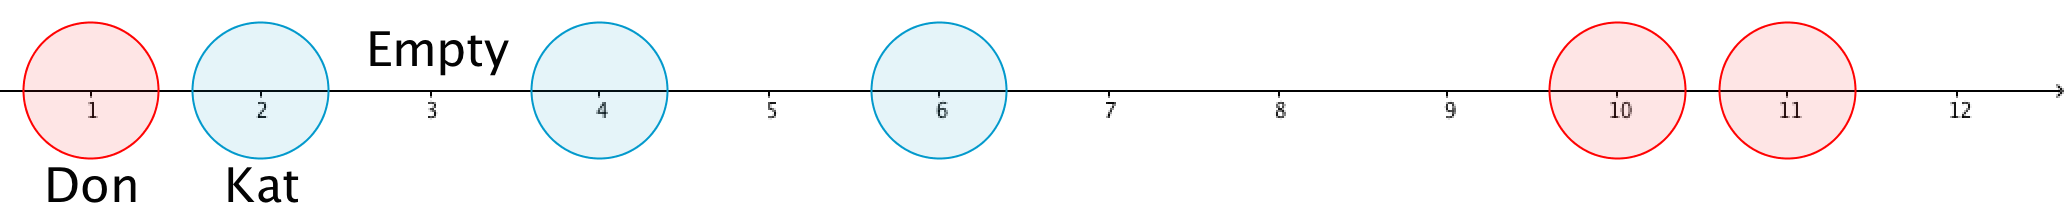
\includegraphics[scale=0.2]{desc.png}
\end{figure}

Pye 希望做出一张正常向的谱面,特别是不能在短时间内出现反复按同一个键的%
要求,因为这样不仅会使得游戏时的音符难以分辨,也会使得对手速,%
甚至键盘的苛刻要求难以满足,进而降低游戏性。因此 Pye 特别关注的数值之一就是%
最近的一对种类相同的音符(Don 与 Don、Kat 与 Kat)所在时刻之差的绝对值。

尽管谱面编辑器并没有提供这个功能,但 Pye 才不需要你的帮助呢!

\subsection*{任务}
给定 Pye 在编辑谱面时的操作顺序,其中包含一系列询问,计算出每个询问的答案。


操作分为以下 4 种:
\begin{itemize}
    \item \texttt{Don <P>}:在时刻 $P$ 的位置放置一个鼓面音符。原来已有的其他音符将被覆盖。
    \item \texttt{Kat <P>}:在时刻 $P$ 的位置放置一个鼓边音符。原来已有的其他音符将被覆盖。
    \item \texttt{Invert <L> <R>}:%
        对于每个满足 $L \leq i \leq R$ 的时刻 $i$:
        \begin{itemize}
            \item 如果时刻 $i$ 的位置上为空,则不进行操作;
            \item 如果时刻 $i$ 的位置上有一个鼓面音符,则将其改为鼓边音符;
            \item 如果时刻 $i$ 的位置上有一个鼓边音符,则将其改为鼓面音符。
        \end{itemize}
    \item \texttt{Inspect <L> <R>}:%
        询问所有满足 $L \leq i \leq R$ 的时刻 $i$ 上的音符中,最近的一对种类相同的音符%
        (Don 与 Don、Kat 与 Kat)所在时刻之差的绝对值。如果这样的一对音符不存在,答案为 -1。
\end{itemize}

\subsection*{输入 \makebox[0.5em]{} \small{obsessed.in}}
\begin{itemize}
    \item 第 $1$ 行:两个正整数 $N$ 和 $M$,分别表示谱面长度和操作数目。
    \item 第 $2 \sim M + 1$ 行:每行描述一个操作,格式与“任务”一节中的描述相同,且所有涉及的数字均为 $[1, N]$ 范围内的正整数。
\end{itemize}

\subsection*{输出 \makebox[0.5em]{} \small{obsessed.out}}
\begin{itemize}
    \item 对于 \texttt{Don}、\texttt{Kat} 和 \texttt{Invert} 操作,不需要进行任何输出;
    \item 对于每个 \texttt{Inspect} 操作输出一行,包括一个整数,表示该次询问的答案。
\end{itemize}

\subsection*{样例}
\begin{table}[h]\centering
\begin{tabularx}{0.8 \textwidth}{|X|X|}
\hline
\texttt{\textbf{obsessed.in}} & \texttt{\textbf{obsessed.out}} \\ \hline
{\ttfamily
10 13\newline
Inspect 3 5\newline
Don 2\newline
Don 4\newline
Inspect 3 5\newline
Inspect 1 5\newline
Kat 3\newline
Kat 6\newline
Inspect 3 10\newline
Inspect 1 10\newline
Invert 3 4\newline
Inspect 1 10\newline
Kat 2\newline
Inspect 2 4
} & {\ttfamily
-1\newline
-1\newline
2\newline
3\newline
2\newline
1\newline
2
}
\\ \hline
\end{tabularx}\end{table}

\subsection*{数据规模与约定}
对于所有子任务,有 $2 \leq N, M \leq 300\,000$。
\subsubsection*{子任务 1 “Kantan” (8 pts)}
\begin{itemize}
    \item $N = 2$。
\end{itemize}
\subsubsection*{子任务 2 “Futsuu” (17 pts)}
\begin{itemize}
    \item $N, M \leq 1\,000$。
\end{itemize}
\subsubsection*{子任务 3 “Inner Oni” (25 pts)}
\begin{itemize}
    \item 没有 \texttt{Kat} 和 \texttt{Invert} 操作。
    \item 所有 \texttt{Don} 操作的 $P$ 值严格单调递增。
\end{itemize}
\subsubsection*{子任务 4 “Muzukashii” (28 pts)}
\begin{itemize}
    \item 没有 \texttt{Invert} 操作。
\end{itemize}
\subsubsection*{子任务 5 “Oni” (22 pts)}
    没有任何附加限制。

\subsection*{限制}
\begin{itemize}
\item 时间:1.0 秒
\item 内存:256.0 MiB
\end{itemize}

\begin{figure}[h]\centering

\includegraphics[scale=0.55]{obsessed.png}
\end{figure}

\end{document}

